%%%%%%%%%%%%%%%%%%%%%%%%%%%%%%%%%%%%%%%%%%%%%%%%%%%%%%%%%%%%%%%%%%%%%%%%%%%%%%%
%
% Filename: template.tex
% Author:   David Oniani
% Modified: January 17, 2020
%  _         _____   __  __
% | |    __ |_   _|__\ \/ /
% | |   / _` || |/ _ \\  /
% | |__| (_| || |  __//  \
% |_____\__,_||_|\___/_/\_\
%
%%%%%%%%%%%%%%%%%%%%%%%%%%%%%%%%%%%%%%%%%%%%%%%%%%%%%%%%%%%%%%%%%%%%%%%%%%%%%%%

%%%%%%%%%%%%%%%%%%%%%%%%%%%%%%%%%%%%%%%%%%%%%%%%%%%%%%%%%%%%%%%%%%%%%%%%%%%%%%%
% Document Definition
%%%%%%%%%%%%%%%%%%%%%%%%%%%%%%%%%%%%%%%%%%%%%%%%%%%%%%%%%%%%%%%%%%%%%%%%%%%%%%%

\documentclass[11pt]{article}

%%%%%%%%%%%%%%%%%%%%%%%%%%%%%%%%%%%%%%%%%%%%%%%%%%%%%%%%%%%%%%%%%%%%%%%%%%%%%%%
% Packages and Related Settings
%%%%%%%%%%%%%%%%%%%%%%%%%%%%%%%%%%%%%%%%%%%%%%%%%%%%%%%%%%%%%%%%%%%%%%%%%%%%%%%

% Global, document-wide settings
\usepackage[margin=1in]{geometry}
\usepackage[utf8]{inputenc}
\usepackage[english]{babel}

% Other packages
\usepackage{booktabs}
\usepackage{hyperref}
\usepackage{mathtools}
\usepackage{amsthm}
\usepackage{amssymb}
\usepackage{tikz}
\usepackage[cache=false]{minted}

%%%%%%%%%%%%%%%%%%%%%%%%%%%%%%%%%%%%%%%%%%%%%%%%%%%%%%%%%%%%%%%%%%%%%%%%%%%%%%%
% Command Definitions and Redefinitions
%%%%%%%%%%%%%%%%%%%%%%%%%%%%%%%%%%%%%%%%%%%%%%%%%%%%%%%%%%%%%%%%%%%%%%%%%%%%%%%

% Nice-looking underline
\newcommand\und[1]{\underline{\smash{#1}}}

% Line spacing is 1.5
\renewcommand{\baselinestretch}{1.5}

% Absolute value
\DeclarePairedDelimiter\abs{\lvert}{\rvert}%

% Absolute value big
\DeclarePairedDelimiter\absb{\Big\lvert}{\Big\rvert}%

% Ceiling
\DeclarePairedDelimiter{\ceil}{\lceil}{\rceil}

% Ceiling big
\DeclarePairedDelimiter{\ceilb}{\Big\lceil}{\Big\rceil}

% Floor
\DeclarePairedDelimiter\floor{\lfloor}{\rfloor}

% % Naturals, Reals, Integers, and Rationals, 
\newcommand{\nats}{\mathbb{N}}
\newcommand{\reals}{\mathbb{R}}
\newcommand{\preals}{\mathbb{R^+}}
\newcommand{\nreals}{\mathbb{R^-}}
\newcommand{\ints}{\mathbb{Z}}
\newcommand{\pints}{\mathbb{Z^+}}
\newcommand{\nints}{\mathbb{Z^-}}
\newcommand{\rats}{\mathbb{Q}}
\newcommand{\prats}{\mathbb{Q^+}}
\newcommand{\nrats}{\mathbb{Q^-}}
\newcommand{\irrats}{\mathbb{I}}
\newcommand{\pirrats}{\mathbb{I^+}}
\newcommand{\nirrats}{\mathbb{I^-}}

%%%%%%%%%%%%%%%%%%%%%%%%%%%%%%%%%%%%%%%%%%%%%%%%%%%%%%%%%%%%%%%%%%%%%%%%%%%%%%%
% Miscellaneous
%%%%%%%%%%%%%%%%%%%%%%%%%%%%%%%%%%%%%%%%%%%%%%%%%%%%%%%%%%%%%%%%%%%%%%%%%%%%%%%

% Setting stuff
\setlength{\parindent}{0pt}  % Remove indentations from paragraphs

% PDF information and nice-looking urls
\hypersetup{%
  pdfauthor={David Oniani},
  pdftitle={Real Analysis},
  pdfsubject={Mathematics, Real Analysis, Real Numbers},
  pdfkeywords={Mathematics, Real Analysis, Real Numbers},
  pdflang={English},
  colorlinks=true,
  linkcolor={black!50!blue},
  citecolor={black!50!blue},
  urlcolor={black!50!blue}
}

%%%%%%%%%%%%%%%%%%%%%%%%%%%%%%%%%%%%%%%%%%%%%%%%%%%%%%%%%%%%%%%%%%%%%%%%%%%%%%%
% Author(s), Title, and Date
%%%%%%%%%%%%%%%%%%%%%%%%%%%%%%%%%%%%%%%%%%%%%%%%%%%%%%%%%%%%%%%%%%%%%%%%%%%%%%%

% Author(s)
\author{David Oniani\\
        Luther College\\
        \href{mailto:oniada01@luther.edu}{oniada01@luther.edu}}

% Title
\title{\rule{\paperwidth - 150pt}{1pt}\textbf{\\\textit{Real Analysis
Exams}\\}\rule {\paperwidth - 150pt}{1pt}\\\textbf{Exam
\textnumero3}\\{\normalsize Instructor: Dr. Eric Westlund}}

% Date
\date{\today}

%%%%%%%%%%%%%%%%%%%%%%%%%%%%%%%%%%%%%%%%%%%%%%%%%%%%%%%%%%%%%%%%%%%%%%%%%%%%%%%
% Beginning of the Document
%%%%%%%%%%%%%%%%%%%%%%%%%%%%%%%%%%%%%%%%%%%%%%%%%%%%%%%%%%%%%%%%%%%%%%%%%%%%%%%

\begin{document}
\maketitle

%%%%%%%%%%%%%%%%%%%%%%%%%%%%%%%%%%%%%%%%%%%%%%%%%%%%%%%%%%%%%%%%%%%%%%%%%%%%%%%

\begin{itemize}
    \item[1.]
        \begin{itemize}
            \item[(a)]
                Yes, it is continuous at $0$. Recall that a function is
                continuous at $x = 0$ if $\lim_{x \to 0}f(x) = f(0) = 0$.
                Notice that $\forall x \neq 0, \abs{\sin{(\frac{1}{x^2})}} \leq
                1$. We then have that $\abs{f(x)} \leq x^4$ (multiply both
                sides of the inequality by $x^4$). Now, since $\lim_{x \to 0}
                x^4 = 0$ and $\lim_{x \to 0} (-x^4) = 0$, it follows by
                \textbf{Squeeze Theorem} that $\lim_{x \to 0} = 0 = f(0)$.
                Hence, $f(x)$ is continuous at $0$.

            \item[(b)]
                Yes, it is differentiable at $0$. Recall that a function is
                differentiable at $x = 0$ if the limit $\lim_{x \to 0}
                \frac{f(x) - f(0)}{x - 0}$ exists. We have:
                \begin{align*}
                    \lim_{x \to 0} \frac{f(x) - f(0)}{x - 0}
                        &= \lim_{x \to 0} \frac{f(x) - 0}{x}\\
                        &= \lim_{x \to 0} \frac{x^4\sin{(\frac{1}{x^2}})}{x}\\
                        &= \lim_{x \to 0} x^3\sin{\Big(\frac{1}{x^2}}\Big)
                \end{align*}
                Now, notice that $x^3\sin{(\frac{1}{x^2})}$ is bounded by
                $-\abs{x^3}$ and $\abs{x^3}$ and once again, by \textbf{Squeeze
                Theorem}, it follows that $f$ is differentiable at $0$.

            \item[(c)]
                $f^\prime(x)$ is continuous at $0$. Away from $0$, we have
                $f^\prime(x) = 4x^3 \sin{(\frac{1}{x^2})} -
                2x\cos{(\frac{1}{x^2})}$. Then $\lim_{x \to 0} f^\prime(x) = 0$
                and thus, $\lim_{x \to 0} f^\prime(x) = 0 = f^\prime(0)$.
                Hence, $f^\prime(x)$ is continuous at $0$.

            \item[(d)]
                No, it is not differentiable at $0$. Recall that a function is
                differentiable at $x = 0$ if the limit $\lim_{x \to 0}
                \frac{f(x) - f(0)}{x - 0}$ exists. We have:
                \begin{align*}
                    \lim_{x \to 0} \frac{f^\prime(x) - f^\prime(0)}{x - 0}
                        &= \lim_{x \to 0} \frac{f(x) - 0}{x}\\
                        &= \lim_{x \to 0} \frac{4x^3 \sin{(\frac{1}{x^2})} -
                            2x\cos{(\frac{1}{x^2})}}{x}\\
                        &= \lim_{x \to 0} 4x^2 \sin{\Big(\frac{1}{x^2}\Big)} -
                            2 \cos{\Big(\frac{1}{x^2}\Big)}
                \end{align*}
                Now, notice that $\lim_{x \to 0} 4x^2
                \sin{\Big(\frac{1}{x^2}\Big)} - 2
                \cos{\Big(\frac{1}{x^2}\Big)}$ does not exist and thus,
                $f^\prime(x)$\ is not differentiable at $0$.
        \end{itemize}

    \item[2.]
        \begin{itemize}
            \item[(a)]
                Since $f(x)$ is differentiable on $[0, 4]$, it is also
                continuous on $[0, 4]$. Now, let $g(x) = f(x) - x$. Then $g$ is
                again both differentiable and continuous on $[0, 4]$. We have
                $g(0) = f(0) = 2$ and $g(4) = f(4) - 4 = -3$. Now, since $g$ is
                continuous, it follows by the \textbf{Theorem 4.5.1
                (Intermediate Value Theorem)} $\exists c \in (0, 4)$ s.t.
                $g(c) = 0$ and for this $c$, we will have $f(c) = g(c) + c = 0
                + c = c$. Hence, $f(x)$ has a fixed point on $[0, 4]$\\
                $\qed$

            \item[(b)]
                Notice that $\frac{f(4) - f(0)}{4 - 0} = \frac{1 - 2}{4} =
                -\frac{1}{4}$. Then it follows by \textbf{Theorem 5.3.2 (Mean
                Value Theorem)} that $\exists c \in (0, 4)$ s.t. $f^\prime(c) =
                -\frac{1}{4}$. On the other hand, we know that $f^\prime(1) =
                2$. Finally, it follows by \textbf{Theorem 5.2.7 (Darboux’s
                Theorem)} that $\exists c \in (0, 4)$ s.t. $f^\prime(c) = 0$.\\
                $\qed$
        \end{itemize}

    \item[3.]
        \begin{itemize}
            \item[(a)]
                For any fixed $x$, we have:
                \begin{equation*}
                    \lim_{n \to \infty} \frac{x^ne^{-x}}{n!}
                        = \lim_{n \to \infty} \frac{x^n}{n!e^x}
                        = 0
                \end{equation*}
                The reason the limit is $0$ is that as $n$ approaches infinity,
                $n!e^x$ grows a lot faster than $x^n$ (one could also use
                \textbf{Squeeze Theorem} to show that the limit is $0$).

            \item[(b)]
                For any fixed $x$, we have:
                \begin{equation*}
                    \abs{g_n(x) - g(x)}
                        = \absb{\frac{x^ne^{-x}}{n!} - 0}
                        = \absb{\frac{x^n}{n!e^x}}
                \end{equation*}
                Now, we need to pick $N$ s.t. $\forall n \geq N$,
                $\absb{\frac{x^n}{n!e^x}} < \epsilon$ holds. Now, although it
                is possible to do for every $x \in [0, \infty)$, there is no
                way to choose a single value of $N$ that will work for all
                values of $x$ at the same time. Thus, such $N$ does not exist.
                Finally, we conclude that the sequence of functions $(g_n)$
                does not uniformly converge to $g$ on $[0, \infty)$.
        \end{itemize}

    \item[4.]
        \begin{itemize}
            \item[(a)]
                \begin{equation*}
                    f^\prime_n(x)
                        = \Big(xe^{-nx^2}\Big)^\prime
                        = e^{-nx^2}(1 - 2nx^2)
                \end{equation*}

            \item[(b)]
                We need to solve the equation $f^\prime_n(x) = 0$.
                We have:
                \begin{equation*}
                    e^{-nx^2}(1 - 2nx^2) = 0 \implies x = \pm \frac{1}{\sqrt{2n}}
                \end{equation*}
                Hence, the global maximum occurs at $x = \frac{1}{\sqrt{2n}}$
                and the global minimum occurs at $x = -\frac{1}{\sqrt{2n}}$.
                \\
                \\
                Let us sketch $f_n(x)$ for $n = 2$. For $n = 2$, we have the
                function $f_2(x) = xe^{-2x^2}$.
                \begin{figure}[H]
                    \centering
                    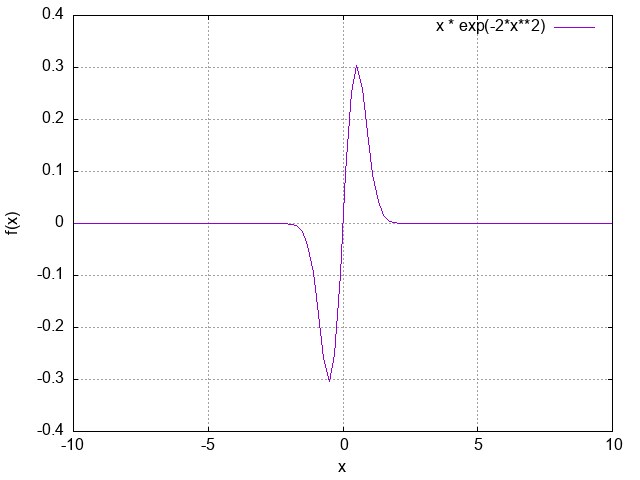
\includegraphics[width=0.7\linewidth]{plot.png}
                    \caption{Plot of $g = xe^{-2x^2}$.}
                \end{figure}

            \item[(c)]
                \begin{align*} 
                    f(x) &= \lim_{n \to \infty} f_n(x)\\
                         &= \lim_{n \to \infty} \Big(xe^{-nx^2}\Big)\\
                         &= \lim_{n \to \infty} \frac{x}{e^{nx^2}}\\
                         &= 0
                     \tag{notice that as $n \to \infty, e^{nx^2} \to \infty$}
                \end{align*} 

            \clearpage

            \item[(d)]
                Since the global maximum of $f(x)$ is $\frac{1}{\sqrt{2n}}$, we
                can let $N = \ceil{\frac{1}{\epsilon^2}}$. Then $\forall n \geq
                N$, we have:
                \begin{equation*}
                    \abs{f_n(x) - f(x)}
                        = \abs{f_n(x)}
                        = \abs{xe^{-nx^2}}
                        \leq \frac{1}{\sqrt{2n}}
                        \leq \frac{1}{\sqrt{2N}}
                        \leq \frac{\epsilon}{\sqrt{2}}
                        < \epsilon
                \end{equation*}
                Now, we could find $N \in \nats$ s.t. $\forall n \geq N,
                \abs{f_n(x) - f(x)} < \epsilon$ holds and hence, $f_n$
                converges uniformly to $f$ on $\reals$.

            \item[(e)]
                \begin{equation*}
                    \lim_{n \to \infty} f^\prime_n(x)
                        = \lim_{n \to \infty} e^{-nx^2}(1 - 2nx^2)
                        = \lim_{n \to \infty} \frac{- 2nx^2 + 1}{e^{nx^2}}
                        = 0
                        \tag{notice that as $n \to \infty, e^n$ grows a lot
                             faster than $2n$}
                \end{equation*}
                Since $f(x) = 0$, it follows that $f^\prime(x) = 0$ and
                finally, we have $f^\prime(x) = \lim_{n \to \infty}
                f^\prime_n(x) = 0$.
        \end{itemize}

    \item[5.]
        \begin{itemize}
            \item[(a)]
                Notice that the following holds:
                \begin{equation*}
                    \absb{\frac{\cos{(3^nx)}}{2^n}} \leq \frac{1}{2^n}
                \end{equation*}
                Now, recall that $\frac{1}{2^n}$ converges (showed many times
                over the course of the class). Then, it follows by
                \textbf{Corollary 6.4.5 (Weierstrass M-Test)} that $g(x) =
                \sum_{n = 1}^\infty \frac{\cos{(3^nx)}}{2^n}$ converges
                uniformly on $\reals$. And since the uniform convergence
                implies continuity, it follows that $g(x) = \sum_{n = 1}^\infty
                \frac{\cos{(3^nx)}}{2^n}$ is continuous on $\reals$.

            \item[(b)]
                Notice that we have:
                \begin{equation*}
                    g^\prime(x) =
                        \sum_{n = 1}^\infty
                            -\Big(\frac{3}{2}\Big)^n\sin{(3^nx)}
                \end{equation*}
                Unfortunately, in this case we cannot apply \textbf{Corollary
                6.4.5 (Weierstrass M-Test)} as $\Big(\frac{3}{2}\Big)^n$ is not
                bounded. Hence, this is the difference between part $(a)$ and
                part $(b)$ of the exercise (we cannot determine if $g$ is
                differentiable on $\reals$).
                \\
                \\
                As a side note, recall that this is the Weierstrass function of
                the form $\sum_{n = 0}^\infty a^n\cos{(b^nx)}$ which is a
                nowhere-differentiable function. Hence, $g^\prime(x)$ is not
                differentiable on $\reals$.
        \end{itemize}

    \item[6.]
        For $x \not\in \mathbb{Q}$, we can show $f_n(x)$ is continuous, since
        for $x < r_n$, we can choose a small enough $\delta$ such that $f_n(y)
        = 0$ for $y \in V_\delta(x)$. Similar logic can be applied when $x >
        r_n$. Now, notice that
        \begin{equation*}
            f_n(x) \leq \frac{1}{2^n}
        \end{equation*}
        Then it follows by \textbf{Corollary 6.4.5 (Weierstrass M-Test)} that
        $f(x)$ converges uniformly.

        Now, since $f_n$ are all continuous, and $f$ converges uniformly, we
        have that $f$ is continuous.

        Furthermore, since every $f_n(x)$ is increasing, $f$ is monotonely
        increasing. Thus, for $x < y$, we get:
        \begin{align*}
          \forall n\ f_n(x) &\leq f_n(y)\\
          \sum_{n = 1}^k f_n(x) &\leq \sum_{n = 1}^k f_n(y)\\
          \lim_k \sum_{n = 1}^k f_n(x) &\leq \lim_k \sum_{n = 1}^k f_n(y)\\
          f(x) &\leq f(y)
        \end{align*}
        Hence, we got that $f$ is increasing on $\reals$.\\
        $\qed$

    \item[7.]
        \begin{itemize}
            % akdjalsk
            \item[(a)]
                We have:
                \begin{align*}
                    \ln (1 + x) &= \sum_{n \geq 1} \frac{f^{(n)} (0)}{n!} x^n\\
                                &= \sum_{n \geq 1}
                                    \frac{(-1)^{n - 1}(n - 1)!}{n!} x^n\\
                                &= \sum_{n \geq 1} \frac{(-1)^{n - 1}}{n} x^n\\
                                &= \sum_{n \geq 1} \frac{(-1)^{n}}{n + 1}
                                   x^{n + 1}\\
                                &= x - \frac{x^2}{3} + \frac{x^3}{3} -
                                       \frac{x^4}{4} + \dots
                \end{align*}
                Hence the taylor series representation is $x - \frac{x^2}{3} +
                \frac{x^3}{3} - \frac{x^4}{4} + \dots$.

            \item[(b)]
                When $x = 1$, we get alternating harmonic series that we know
                converges [shown many times over the course of the class]. It
                diverges when $x = -1$ as we get the $-\frac{1}{n}$ which is
                the negative harmonic series that we know diverges [shown many
                times over the course of the class]). Then it follows that the
                series converges when $-1 < x \leq 1$. Hence, the interval of
                convergence of the series is $(-1, 1]$ (the radius of
                convergence is $1$).

            \item[(c)]
                Yes, it does. Let us apply the ratio test. We get:
                \begin{equation*}
                    \lim_{n \to \infty} \frac{\frac{(-1)^{n + 1}}{n + 2} x^{n +
                    2}}{\frac{(-1)^{n}}{n + 1} x^{n + 1}} = -\frac{n + 1}{n +
                    2} x = -x
                \end{equation*}
                Note that the series converges uniformly if $\abs{-x} = \abs{x}
                < 1$. Hence, it converges on $(-1, 1)$. We now need to check
                the endpoints $x = -1$ and $x = 1$. Notice that if $x = -1$,
                the series does not converge uniformly as $\ln (1 + -1) = \ln
                (0)$ which is undefined (negative infinity). For $x = 1$, it
                follows by \textbf{Leibnitz’ test for alternating series}, that
                the series converges. Hence, the Taylor series converges
                uniformly to $f$ on $(-1, 1]$ which is its interval of
                convergence.
        \end{itemize}
\end{itemize}

%%%%%%%%%%%%%%%%%%%%%%%%%%%%%%%%%%%%%%%%%%%%%%%%%%%%%%%%%%%%%%%%%%%%%%%%%%%%%%%
% The End of the Document
%%%%%%%%%%%%%%%%%%%%%%%%%%%%%%%%%%%%%%%%%%%%%%%%%%%%%%%%%%%%%%%%%%%%%%%%%%%%%%%

\end{document}
